\section{Introduction}

%The cardiovascular system and its components have been vastly studied and a lot 
%of visualization techniques to study the heart or the arteries of the human body 
%have  been  proposed.  In  this  STAR  report,  you  need  to  conduct  a  survey  on 
%important  medical  visualization  applications  that  cover  the  topic  of 
%cardiovascular visualization, to propose a taxonomy of the existing applications, 
%and to provide an overview of yet-unaddressed or challenging topics.  

% Intro from MedVis book
For diagnosis as well as for therapy planning it is crutial to understand the branching pattern and morphology of tree-like anatomical structures \cite{preim2013visual}.
Depending on the capturing technique we are confronted with 3D data that could have very high spacial or temporal resolution. The visual analysis of this static or dynamic data is a challanging task.

\begin{figure}[h]
	\centering
	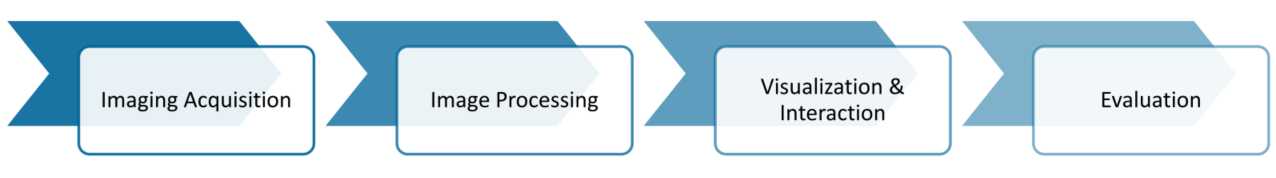
\includegraphics[width=0.4\textwidth]{./Images/MedicalVisualizationPipeline.png} \\
	\caption{Medical visualization pipeline.}
	%\cite{volkau2005geometric}
	\label{fig:MedicalVisualizationPipeline}
\end{figure}

The medical visualization pipeline shown in figure \ref{fig:MedicalVisualizationPipeline} serves as orientation how vascular structures are visualized. We are actually focusing on 3D image processing and visualization. The interested reader will find a complete survey of the whole pipeline for instance in \cite{preim2013visual}. 

Our goal here is to describe methods that visualize vascular structures. Our initial interest is how to separate this structures from background data. Direct volume rendering techniques can be used to visualize this enhanced and visually seperated data. If a more concrete separation is necesarry we have to switch to surface visualization techniques.
There we first have to do segmentation and centerline extraction at the 3D image processing stage. Further the possible visualization techniques spilts in \emph{model-based} and \emph{model-free} approaches. 
Model-based mesh generation follows some more restrictive assumption about the vascular struture whereas model-free mesh generation tries to capture as much original information as possible.


\subsection{Taxonomy}

